\chapter{Results}
\label{cha:results}
In this chapter we will discuss the identified model generated by the
\Autoref{alg:identification} using different values of $k$, taking
on account the number of paths extracted from the \verb|.csv| file and the
number of states generated by the identification algorithm.

\section{Identified Model}
As it was discussed in \Autoref{cha:background}, in this work we assume that all
sequences of events that have length $n_0+1$ were observed, so 
$L_{OrigNI}^{\leq n_0}=\emptyset$ can be true. In order to observe this
sequences of events, the acquisition should by made for a sufficiently
long time, thus the dataset was acquired from an experiment that lasted for 2
hours completing the cycle of filling the rack from top to bottom  4 times and a
half. A time lapse of the process can be seen in
\url{https://www.youtube.com/watch?v=ZtCCKJtA9pI}.

The acquisition started once the system was initialised, that means,
when the system is ready to begin the process, this correspond to place
\hyperlink{partialTable:p27}{$p_{27}$} in \Autoref{fig:petriInitialization}.

The collected data\footnote{Available at:
  \url{https://raw.githubusercontent.com/Accacio/docsTCC/master/data/2019-05-10/2019-05-10_1524.csv}}
of this experiment that lasted for 2 hours has 19751 entries using 65
variables, the inputs\slash outputs of the system and the auxiliary variables
\verb|ConcUP| and \verb|ConcDWN|.

Once this data was collected, the paths were extracted from the \verb|.csv| and the
result was kind of unexpected. The total number of paths using this raw data is equal to
2. This result can be easily explained by the behaviour of the system. As it is
formed by different models, and some work simultaneously with others, the system
has an important parallel behaviour. As these modules are not necessarily
synchronised, it is very unlikely that all of them will return to their initial
state at the same time, resulting in a few very long paths. 


As expected, with a greater value of $k$, more states are identified, the
\Autoref{fig:statesIdentOriginal} show the variation of the number of
states by changing the value of $k$.
\begin{figure}[H]
  \centering
  \includegraphics[width=0.5\textwidth]{results/all/states.pdf}
  \caption{Number of states of identified model for different values of $k$.}
    \label{fig:statesIdentOriginal}
\end{figure}

As seen, the number of states for all values of $k$ is greater than $1000$. Models of this magnitude are very difficult to depict in state transition
diagrams for two reasons; the legibility of such image would be terrible and the
effort to draw it would be very time consuming (drawing it manually) or resource
intensive (drawing using an automated tool). The automated tool known for drawing
graphs has an upper bound aroud 350 nodes, so a tool was developed to
automatically generate the list of \ffunction{} functions of the identified model.

The  list of \ffunction{} functions generated using the original \verb|.csv| file
for $k=1$ and $k=2$
can be seen in  
\url{https://raw.githubusercontent.com/Accacio/docsTCC/master/figures/results/all/flistk1.tex}
% \Autoref{sec:originalKone}
and
\url{https://raw.githubusercontent.com/Accacio/docsTCC/master/figures/results/all/flistk2.tex}
% \Autoref{sec:originalKtwo}
respectively.

We can also make a comparison between the exceeding language generated by the
identified model using the \DAOCT{} model and the \NDAAO{} model, proposed by
\cite{klein2005fault}. This comparison can show that even for a considerable
large system with more than 60 inputs\slash outputs, the \DAOCT{} is more
tailored for fault detection, as the cardinality of its exceeding language is
inferior to that of a \NDAAO{} model of the same size (with a similar \ffunction{} function).

The \Autoref{fig:daoctNdaaoOriginal} shows this comparison using 2 values of $k$.
In this case if we take, for example, $k=1$ and $n=12$ the
exceeding language of \NDAAO{} is $1018$ and for \DAOCT{} it is $923$. And
if we take $k=2$, both are $0$ for $n\leq12$. This mean in this case, with very
long paths, both have a similar behaviour, but \DAOCT{} still have a smaller exceeding language.
\begin{figure}[H]
  \centering
  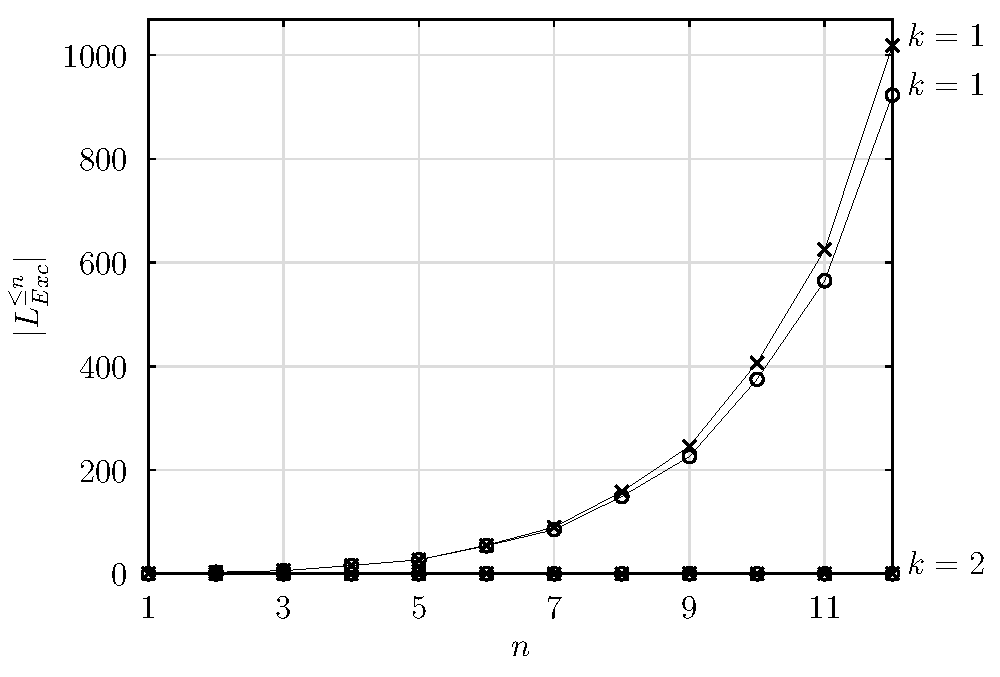
\includegraphics[width=0.5\textwidth]{results/all/exceedingLanguage-daoct-ndaao_k1-2_n12.pdf}
  \caption{Comparison between the cardinality of the exceeding language generated by the DAOCT (o) and
NDAAO ($\times$) models, for $k=1$ and $k=2$.}
    \label{fig:daoctNdaaoOriginal}
\end{figure}

% \subsection{best}
Since the original \verb|.csv| file only could get only 2 paths extracted, an
experiment was made in order to increase the number of paths and see how
different the generated model would be.

The file was processed by a tool, where all vectors
were sorted by the number of duplicates in the file. The vector with most
duplicates was elected to be the new initial vector, consequentially the initial
state of the new model.

A new \verb|.csv| file was created from the original one. It was created by
discarding all vectors from the beginning of the file up to the
first appearance of the new initial vector, so this vector could be the first
one to be processed in the path extraction.

Instead of the original 19751 entries, the new
file 
had 19427 entries. This difference in number entries can be reflected in the number of
generated states.

This new file, after the path extraction, resulted in 80 paths, 40 times the
number of paths of the original.  

Similarly to \Autoref{fig:statesIdentOriginal}, \Autoref{fig:statesIdentBest}
shows the variation of number of states with respect of the values of $k$. This
figure can be used to see the relation
between the change in the number of entries on the \verb|.csv| file and the
number of generated states.
\begin{figure}[H]
  \centering
  \includegraphics[width=0.5\textwidth]{results/all/best/states.pdf}
  \caption{Number of states of identified model for different values of $k$.}
    \label{fig:statesIdentBest}
\end{figure}
Although both figures seem similar, both have the same order of magnitude for
each $k$, the number of states diverges. If we put the values in a vector we can
compare them. While for the original file the corresponding vector is
$\colvec{1321& 2166& 2962& 3744& 4508& 5235& 5939}$, for the modified is 
$\colvec{1294& 2127& 2904& 3663& 4395& 5088& 5746}$.
This change can be caused, as said, by the difference in the number of entries
in the \verb|.csv| files.

Similarly, the list of \ffunction{} functions generated using the modified \verb|.csv| file
for $k=1$ and $k=2$
can be seen in  
\url{https://raw.githubusercontent.com/Accacio/docsTCC/master/figures/results/all/best/flistk1.tex}
% \Autoref{sec:bestKone}
and
\url{https://raw.githubusercontent.com/Accacio/docsTCC/master/figures/results/all/best/flistk2.tex}
% \Autoref{sec:bestKtwo}
respectively.

The same comparison between the \DAOCT{} and \NDAAO{} was made and is shown in \Crefrange{fig:daoctNdaaoBestkone}{fig:daoctNdaaoBestkthree}.

In this second case we can see that the difference between the language of the \DAOCT{} and
\NDAAO{} models is more substantial. For example, for $k=1$ and $n=12$ the
exceeding language of \NDAAO{} is $465332$ and for \DAOCT{} it is $24866$. For
$k=2$ and $n=12$, it is $1943$ and $3$, for \NDAAO{} and \DAOCT{} respectively. And
if we take $k=3$ and $n=12$, it is $712$ for \NDAAO{} and $0$ \DAOCT{}. With
smaller and more numerous paths, we can see more clearly the difference between the
exceeding language of the models. For instance if we want to detect correctly
the failures of the system for sequences of length equal to or smaller
than $12$, using the \DAOCT{} model it is needed only to use a $k=3$ while for the
\NDAAO{} it is needed to use a $k$ greater than 7, for $k=7$ and $n=12$ the
exceeding language of \NDAAO{} is still equal to $47$. Showing that \NDAAO{} is more
computationally expensive for the identification of a system.

\begin{figure}[H]
  % \centering
  \begin{subfigure}[H]{0.5\textwidth}
    \centering
    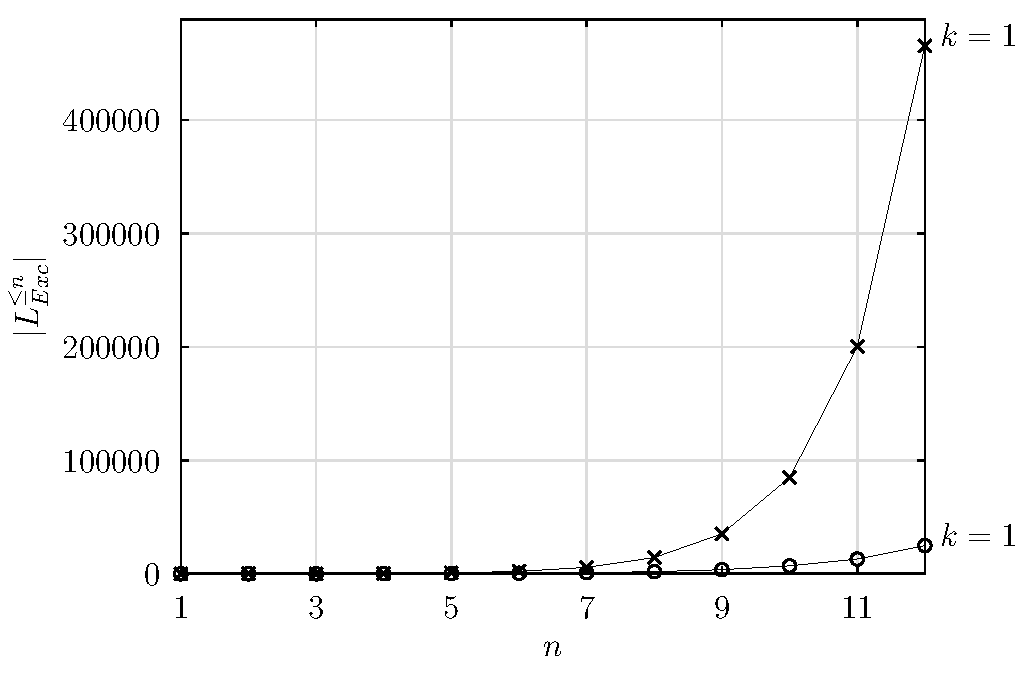
\includegraphics[width=\textwidth]{results/all/best/exceedingLanguage-daoct-ndaao_k1_n12.pdf}
    \caption{$k=1$}
    \label{fig:daoctNdaaoBestkone}
  \end{subfigure}
  ~
  \begin{subfigure}[h]{0.5\textwidth}
    \centering
    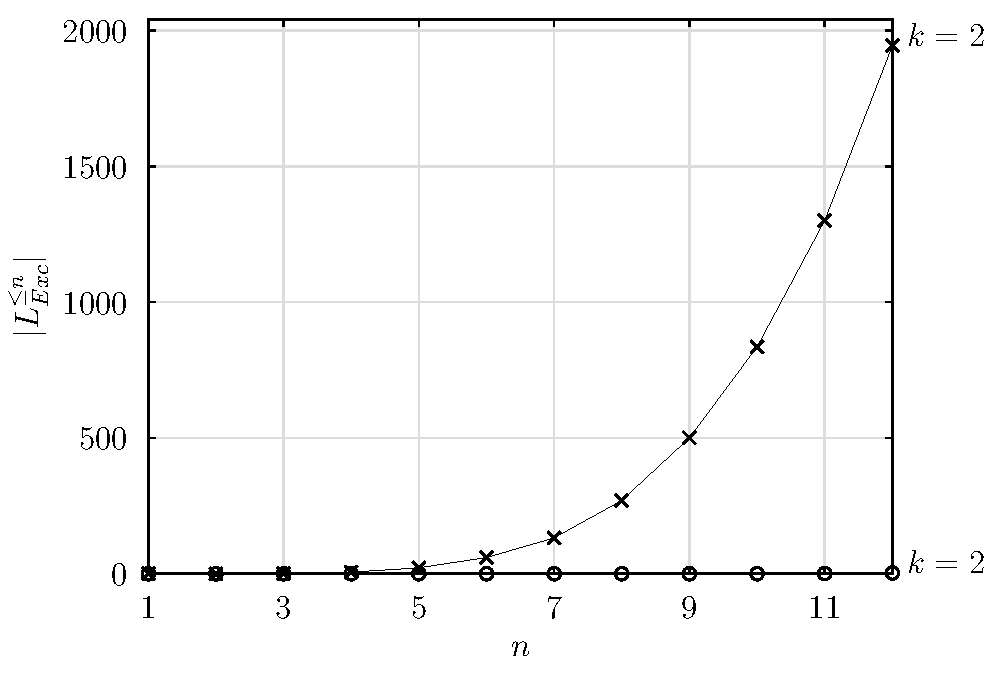
\includegraphics[width=\textwidth]{results/all/best/exceedingLanguage-daoct-ndaao_k2_n12.pdf}
    \caption{$k=2$}
    \label{fig:daoctNdaaoBestktwo}
  \end{subfigure}
  % \begin{center}
  \begin{subfigure}[h]{0.5\textwidth}
    \centering
    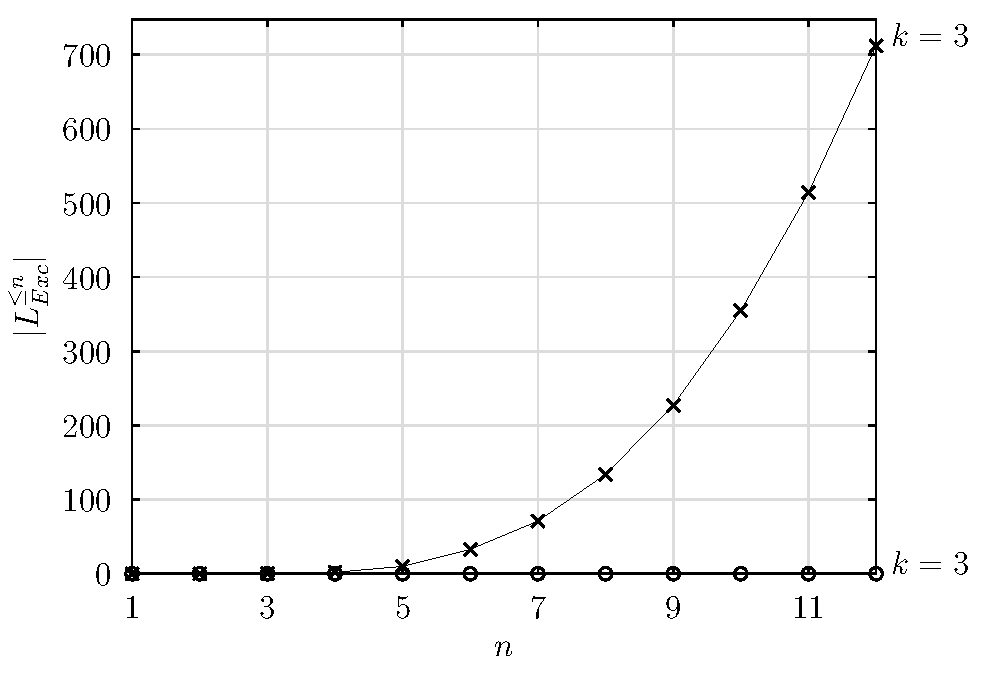
\includegraphics[width=\textwidth]{results/all/best/exceedingLanguage-daoct-ndaao_k3_n12.pdf}
    \caption{$k=3$}
    \label{fig:daoctNdaaoBestkthree}
  \end{subfigure}
  \begin{subfigure}[h]{0.5\textwidth}
    \centering
    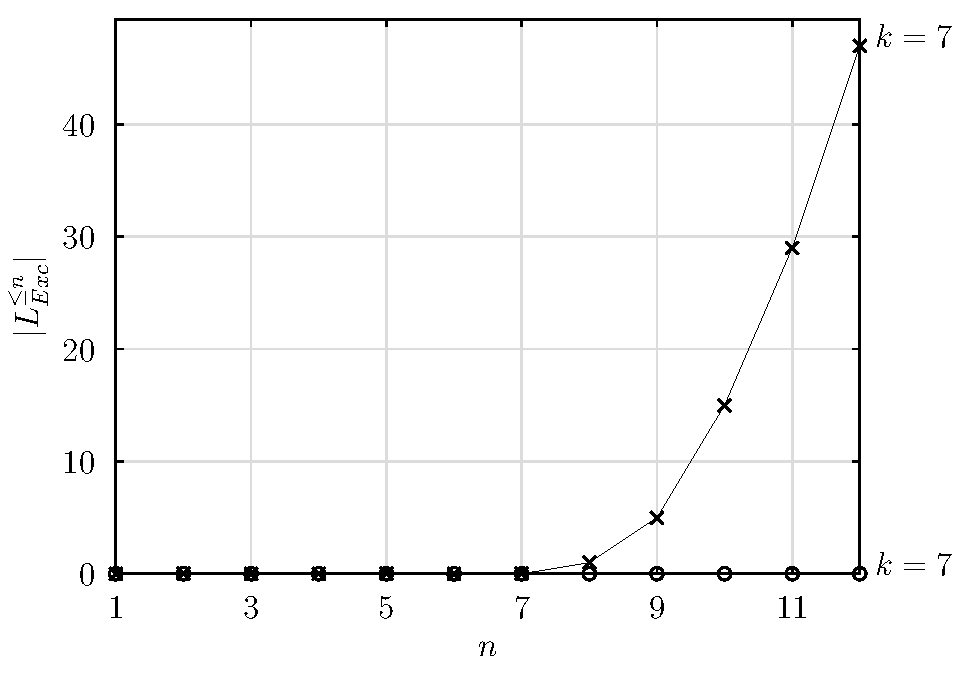
\includegraphics[width=\textwidth]{results/all/best/exceedingLanguage-daoct-ndaao_k7_n12.pdf}
    \caption{$k=7$}
    \label{fig:daoctNdaaoBestkseven}
  \end{subfigure}
    % \end{center}
  \caption{Comparison between the cardinality of the exceeding language generated by the DAOCT (o) and
NDAAO ($\times$) models.}
\end{figure}
Although the modified \verb|.csv| generates more paths and shows a more
considerable difference in the exceeding language generated by both models, the
change of initial vector does not mean that it creates a more trustworthy model,
that it represents better the
system. The choice of this first vector of acquisition will discussed in the
next section in the form an example.
\newpage
\section{About the choice of the first vector}
Let us take as an example the following system: 
\begin{example}[Conveyor Belt with 3 sensors]~\\
  \label{ex:conveyor}
 This simple system consists in a conveyor belt with three sensors $S_1$, $S_2$ and
 $S_3$. A scheme of the conveyor and its sensors can be seen in
 \Autoref{fig:schemeExConveyor}. This conveyor is used to transport boxes, from
 the left to the right.  The boxes are placed one at a time, so only a box can be
 over the conveyor, as it was a requisite for the design of the control. Once the box is over
 the conveyor and begin to be transported, it activates and deactivates $S_1$,
 then activates and deactivates $S_2$ and
 finally activates and deactivates $S_3$. After $S_3$ is deactivated another
 system know that the conveyor is empty and then it puts another box over the
 conveyor belt to restart its cycle. Since only a box is placed over the belt,
 it is impossible to 2 sensors to be activated the same time. And as the belt is always turned on, this system
 only has outputs (inputs to the controller), that are the signals of the three sensors $S_1$, $S_2$ and
 $S_3$.
\end{example}
\begin{figure}[H]
  \centering
  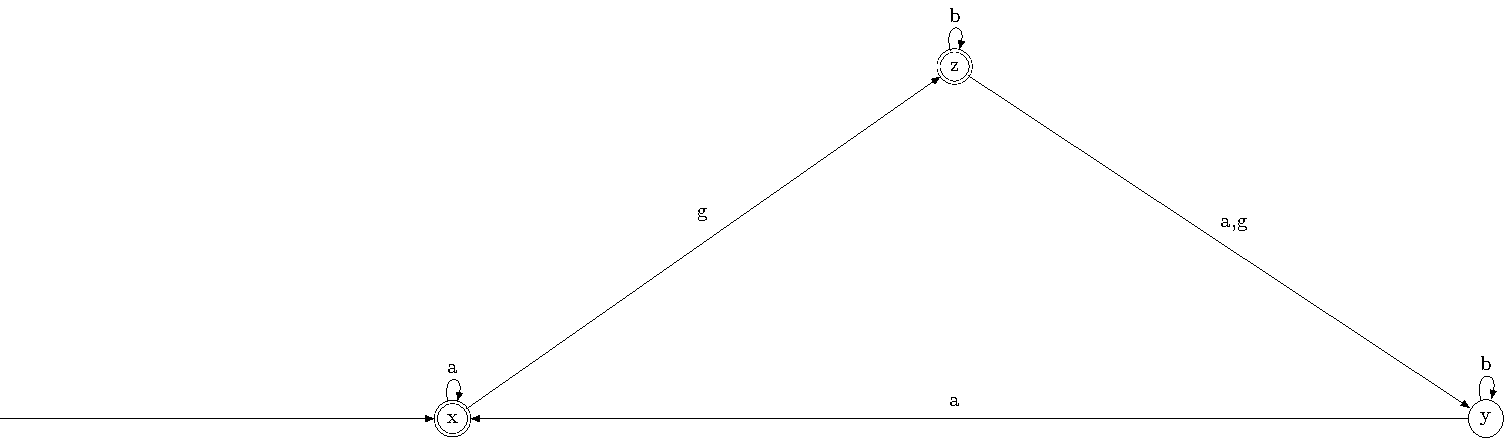
\includegraphics{results/example/example}
  \caption{Scheme of the example \ref{ex:conveyor}.}
    \label{fig:schemeExConveyor}
\end{figure}
If we make the data acquisition of this system and compose a vector with the
values of $S_1$, $S_2$ and $S_3$, we will have the following repeating motif:
\begin{align}
  \label{motif}
\colvec{0\\0\\0}\colvec{1\\0\\0}\colvec{0\\0\\0}\colvec{0\\1\\0}\colvec{0\\0\\0}\colvec{0\\0\\1}
\end{align}
This motif will be repeated multiple times on the \verb|.csv| file forming
cycles, and since it forms cycles the motif can be rewritten in how many ways as
it has vertices, in this case it can be written in 6 ways. To reduce the
complexity we will only discuss 2 ways of writing it, the first one shown in
\ref{motif} and the second shown in \ref{motifMod}. So, we can define two datasets of acquisition,
one beginning with $\colvec{0&0&0}^T$ and other with $\colvec{1&0&0}^T$.
\begin{align}
  \label{motifMod}
\colvec{1\\0\\0}\colvec{0\\0\\0}\colvec{0\\1\\0}\colvec{0\\0\\0}\colvec{0\\0\\1}\colvec{0\\0\\0}
\end{align}
If we take the first dataset, the one beginning with $\colvec{0&0&0}^T$ and
input it in the identification algorithm, the identified model, for $k=1$ can be
seen in \Autoref{fig:exampleCol000k1}. 
\begin{figure}[H]
  \centering
 \includegraphics{results/example/examplek1NoArrows}
  \caption{Identified model using $\colvec{0&0&0}^T$ as initial state, $k=1$.}
    \label{fig:exampleCol000k1}
\end{figure}
As we can see in the arcs of the state transition diagram, three paths were
extracted, this is caused by the way the motif is constructed. As
$\colvec{0&0&0}^T$ is considered the first vector and it repeats thrice
throughout the motif, every time it is repeated another path is created.

But if we take the second dataset instead, the one beginning with $\colvec{1&0&0}^T$ and
input it in the identification algorithm, the identified model, for $k=1$ can be
seen in \Autoref{fig:exampleCol100k1}. 
\begin{figure}[H]
  \centering
  \includegraphics{results/example/example1k1NoArrows}
  \caption{Identified model using $\colvec{1&0&0}^T$ as initial state, $k=1$.}
    \label{fig:exampleCol100k1}
\end{figure}
As we can see only one path is created this time. In this figure we can see the
representation of the vector $\colvec{0&0&0}^T$ as a central hub, the state
$x_1$ in this state transition diagram, where all other states have arcs coming
from or going to it. If we use a greater value of $k$, take $k=2$, for instance, we can have a
better vision of this unique path, see \Autoref{fig:exampleCol100k2}.
\begin{figure}[H]
  \centering
  \includegraphics{results/example/example1k2NoArrows}
  \caption{Identified model using $\colvec{1&0&0}^T$ as initial state, $k=2$.}
    \label{fig:exampleCol100k2}
  \end{figure}

  In the first case, using $\colvec{0&0&0}^T$ as the initial vector, two more
  paths were created when comparing with the second case, where
  $\colvec{1&0&0}^T$ is used as the initial state. At a first glance it could
  seem that these 2 additional paths increase the information we have about the system,
  but actually, it does not. If we take the allowed
  sequences on this first case, we can see that the events $\uparrow 2$ and
  $\uparrow 3$ are allowed even before the event $\uparrow 1$ is triggered,
  which is not part of the normal functioning of the system, described in
  example \Autoref{ex:conveyor}.

  So, even with only one path, the second case, using $\colvec{1&0&0}^T$ as
  initial state, represents better the system, since $\colvec{1&0&0}^T$ happens
  only once in the motif making the extracted path to store almost all the
  sequence of events described in example \Autoref{ex:conveyor}.

  As we can see the choice of the first vector plays a very important part on
  the
  extraction of paths and the assignment of the initial state of the identified
  system.
  \begin{observation}
  An important remark to make is to show that we could only tell
  which identified system was more trustworthy because of the description of
  example \ref{ex:conveyor}. But once we have some information about the system,
  the approach ceases to be a black box one to be a grey box approach. 
\end{observation}

This remark shows that the success of the \DAOCT{} model is very dependent on a good
choice of the initial vector, and consequentially the initial state of the
system. But a question remains for a future work, how can we be sure if the
initial state was well chosen once we do not know any of the system original behaviour?
Maybe this kind of problem resides on the fact that input\slash output vectors
are used to extract the paths and to create the events. An answer could be
making it the other way around, developing an identification model that uses purely
the events. The events are acquired in the first place and then they are used to
extract the paths, and consequentially to identify the system.
%%% Local Variables:
%%% mode: latex
%%% TeX-master: "../monografia"
%%% End:
